\chapter{Coleta de Dados}

Nas próximas seções, apresentaremos quais dados utilizamos neste trabalho para treinar e validar os modelos e como eles foram coletados. 
  
% \section{Área de Estudo}

% A mesorregião do Extremo Oeste da Baiano, na Bahia, é composta por 24 municípios que representam, juntos, uma área de aproximadamente 11,7 Mha (Figura \ref{fig:area_de_estudo}). A área destinada à atividade agrícola, entre os anos de 1985 e 2020, teve uma expansão de mais de 10 vezes, passando de 201.155 ha em 1985 para 2.275.160 ha em 2020, segundo os dados da pesquisa de Produção Agrícola Municipal (PAM), do Instituto
% Brasileiro de Geografia e Estatística (IBGE) \cite{ibge2021pam}. Os principais produtos cultivados são: soja, milho, algodão, e feijão, além de alguns cultivos frutíferos.

% \begin{figure}[H]
% \centering
% \caption{Representação da mesorregião do Extremo Oeste da Bahia, área de estudo utilizada como o foco deste trabalho.}
% \label{fig:area_de_estudo}
% 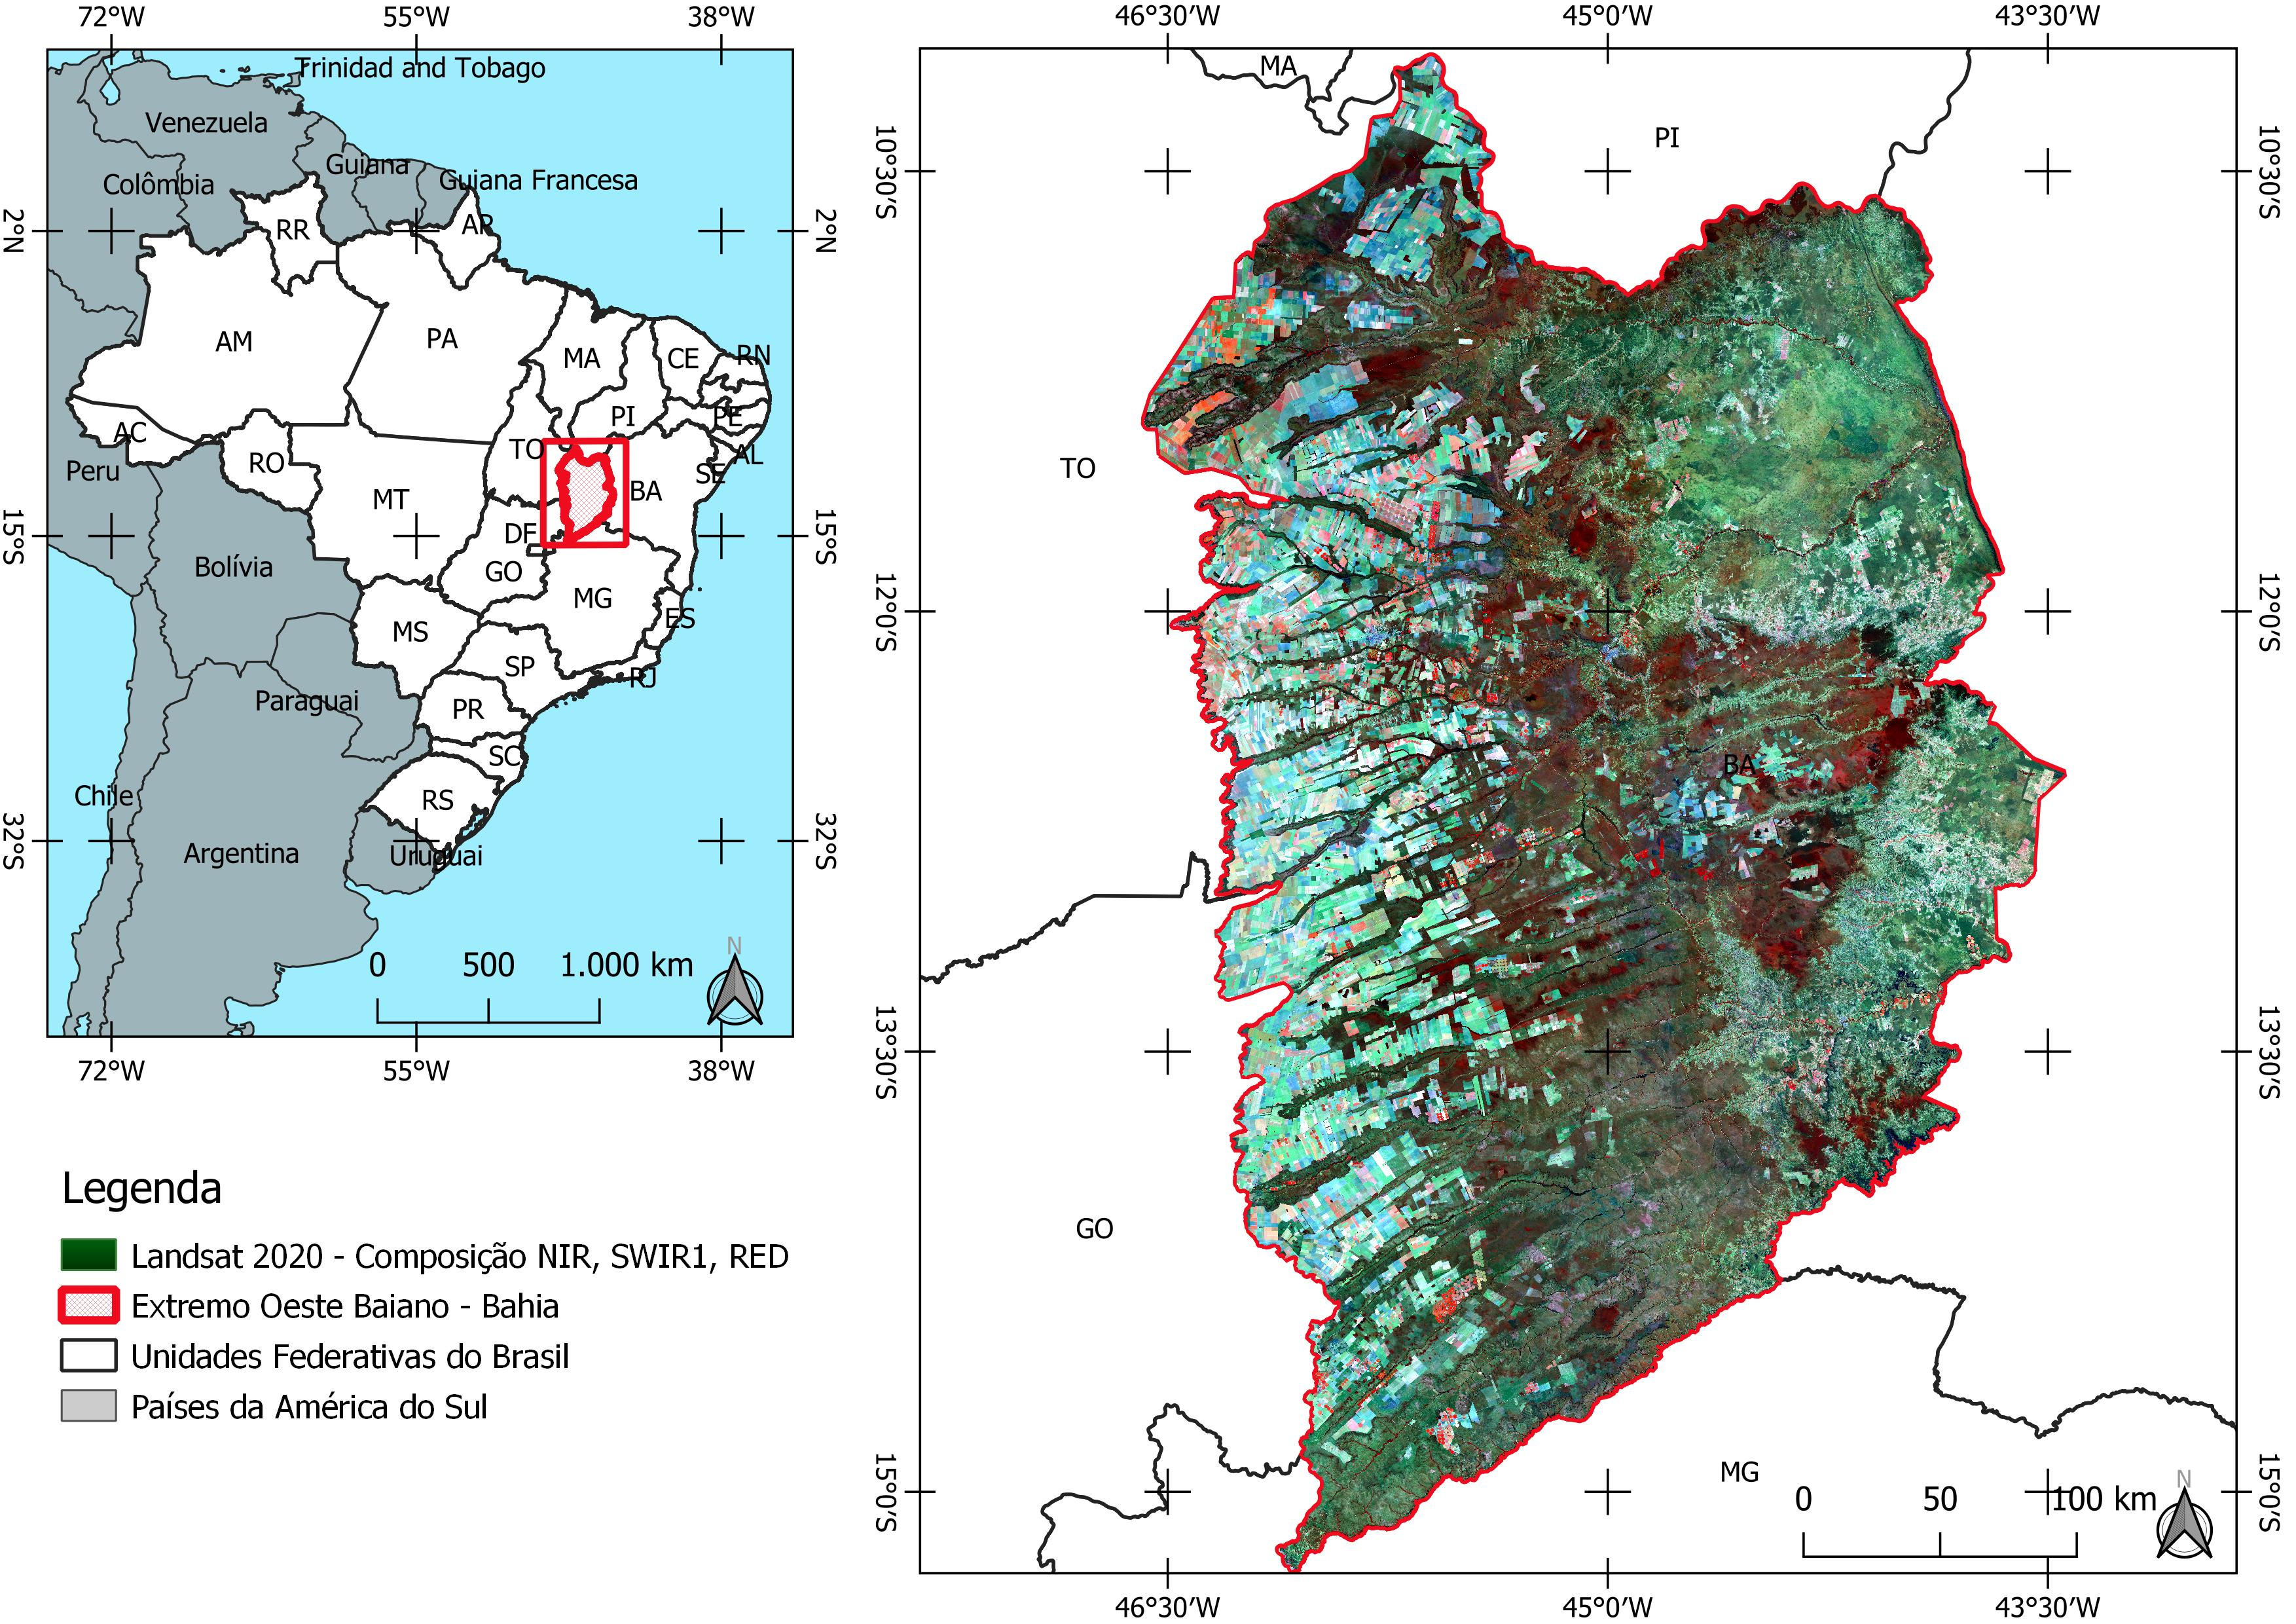
\includegraphics[width=0.6\textwidth]{figuras/area_de_interesse.jpg}
% \end{figure}

\section{Dados de Referência}

Um dos grandes desafios no mapeamento do uso e cobertura da terra é encontrar dados de referência de qualidade com o conjunto de características que se deseja estudar. Neste trabalho, utilizamos dois conjuntos de dados produzidos pelo Instituto Nacional de Pesquisas Espaciais (INPE) em parceria com a Pontifícia Universidade Católica do Rio de Janeiro (PUC Rio), o LEM Dataset e seu sucessor chamado LEM+ Dataset (Tabela \ref{tab:conjunto_de_dados}). O LEM Dataset foi construído após dois trabalho de campo realizados no município de Luís Eduardo Magalhães (LEM), na Bahia, entre junho de 2017 e março de 2018, período correspondente a segunda (estação seca) e a primeira (estação chuvosa) safra brasileira, respectivamente. já o LEM+ Dataset reúne dados coletados de outubro de 2019 a setembro de 2020 (um ano agrícola brasileiro) de Luís Eduardo Magalhães e outros municípios no oeste do estado da Bahia.    

\begin{table}[H]
\caption{Dados contendo os polígonos e as classes que foram utilizados como referência (\textit{Ground truth}) para este trabalho.}
\label{tab:conjunto_de_dados}
\begin{adjustbox}{width=\textwidth}
\begin{tabular}{|l|l|l|l|l|}
\hline
Conjunto de dados & Início     & Fim        & Área Mapeada & Referência \\ \hline
LEM Dataset       & 01/06/2017 & 31/05/2018 & 56.983 ha    & \cite{sanches2018lem} \\ \hline
LEM+ Dataset      & 01/10/2019 & 30/09/2020 & 251.038 ha   & \cite{oldoni2020lem}  \\ \hline
\end{tabular}
\end{adjustbox}
\begin{tablenotes}
\item[1] Os dados do LEM Dataset foram baixados em \url{http://www.dpi.inpe.br/agricultural-database/lem/dados/shp/classes_mensal_LEM_buffer_cut_v2.zip}, acesso em 01/08/2021. \\
\item[2] Os dados do LEM+ Dataset foram baixados em \url{https://md-datasets-public-files-prod.s3.eu-west-1.amazonaws.com/e0bd4285-03b8-494b-bc4d-fc89d80e6bd0}, acesso em 01/08/2021.
\end{tablenotes}
\end{table}

Com base em informações coletadas em campo, sensoriamento remoto óptico de imagens de séries temporais (Sentinel 2A e 2B / MSI e Landsat-8 / OLI) e perfis de NDVI (MODIS/Terra), os analistas conseguiram produzir esses dois conjuntos de dados que possibilitaram acompanhar, mensalmente, as mudanças de uso e cobertura da terra para os ano-safra em que ocorreram esses trabalhos de campo. A Figura \ref{fig:serie_imagens_exemplo_lemdataset} apresenta um exemplo de como estão organizados os dados de referência.  

\begin{figure}[H]
    \centering
    \caption{Exemplo de uma série temporal imagens de satélite em composição falsa cor (NIR, SWIR1, red) (a) e o índice de vegetação NDVI MODIS (b) usado para mapear, mensalmente, a classe de uso da terra  para as coordenadas -45,739369 e -12,156452 (lon, lat) no período de 01/10/2019 à 30/09/2020.}
    \label{fig:serie_imagens_exemplo_lemdataset}
    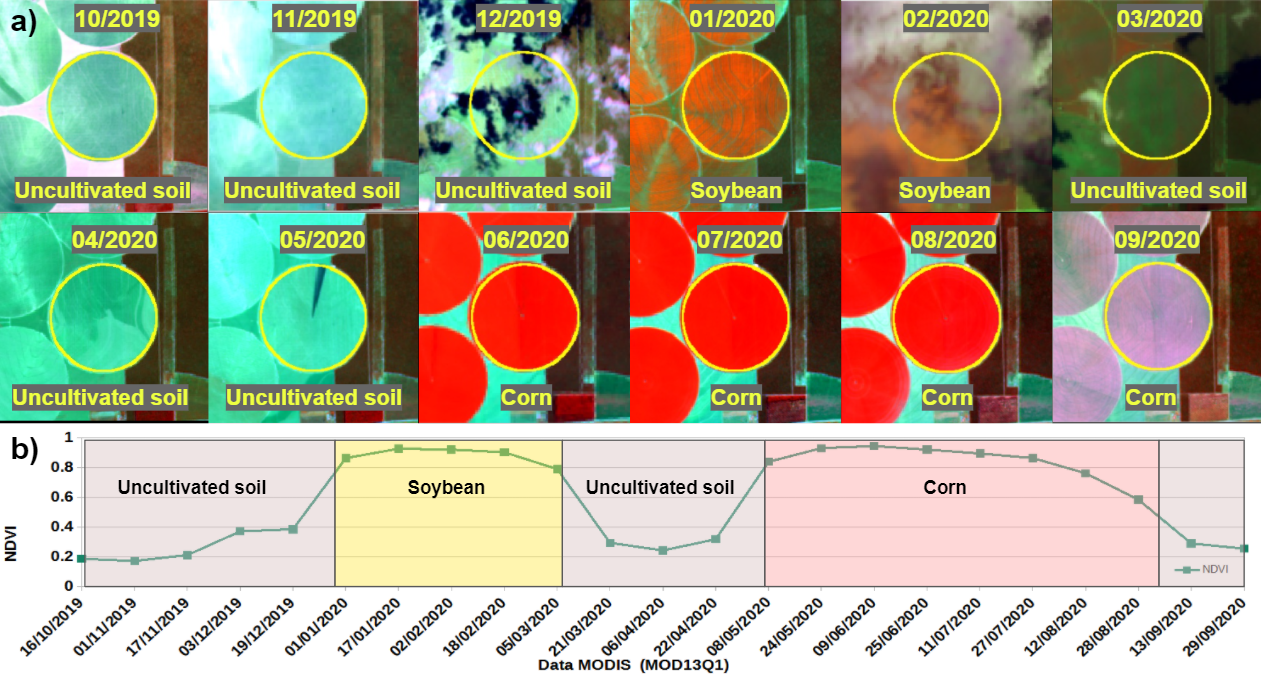
\includegraphics[width=0.7\textwidth]{figuras/exemplo_serie_temporal.png}
\end{figure}


\section{Imagens de satélite}

As imagens que utilizamos neste trabalho foram obtidas dos satélites Landsat 8 (sensor OLI), que possui como provedor oficial das imagens o serviço geológico dos Estados Unidos (USGS), e os satélites Sentinel 2A e 2B (sensor MSI) que são administrados pela Agência Espacial Europeia (ESA). 

A USGS disponibiliza as imagens do satélite Landsat 8 em duas diferentes coleções de imagens, a \textit{Collection 1} e a \textit{Collection 2} \cite{eros2017landsat}. As imagens disponíveis da \textit{Collection 2} possuem um maior nível de qualidade e correções. Por este motivo, neste trabalho utilizamos apenas as imagens disponíveis na \textit{Collection 2}. As imagens disponíveis na \textit{Collection 2} são agrupadas em dois diferentes níveis de qualidade, \textit{Tier 1} e \textit{Tier 2}  \cite{eros2017landsat}. As imagens disponíveis no \textit{Tier 1} são imagens com maior qualidade e Erro Quadrático Médio (RMSE) de registro menor ou igual a 12 metros \cite{eros2017landsat}, já as imagens disponíveis no \textit{Tier 2} possuem RMSE de registro maior que 12 metros. Neste trabalho, processamos apenas as imagens disponíveis no \textit{Tier 1} da \textit{Collection 2}.

A ESA disponibiliza as imagens dos satélites Sentinel 2A e 2B em diferentes níveis de processamento, \textit{Levels} 0, 1 e 2 \cite{sentinel2user}. As imagens do \textit{Level-2} possuem maior nível de processamento e ajustes, porém a ESA não processa e disponibiliza todas as imagens neste nível de processamento. Por este motivo, neste trabalho utilizamos apenas as imagens Sentinel 2A e 2B disponíveis no \textit{Level-1} de processamento. O \textit{Level-1} de processamento das imagens Sentinel 2A e 2B possui três subníveis de processamento, são eles: o \textit{Level-1A}, \textit{Level-1B} e \textit{Level-1C} \cite{sentinel2user}. O \textit{Level-1C} apresenta, além de todas as correções dos níveis \textit{Level-1A} e \textit{Level-1B}, também correção radiométrica e geométrica, o que nos levou a escolhê-lo para obter as imagens Sentinel 2A e 2B utilizadas neste trabalho.    

Os períodos que escolhemos para a obtenção das imagens foram: de 01/06/2017 à 31/05/2018, de 01/10/2019 à 30/09/2020 e de 01/10/2020 à 30/09/2021. Os dois primeiros períodos foram escolhidos baseados nos dados de referência, e o último período foi escolhido para testar o mapeamento em dados mais recentes. Sendo assim, utilizamos as imagens obtidas nos dos primeiros períodos para o treinamento e validação do modelo, e as imagens obtidas no último período para verificar o resultado do modelo em imagens mais recentes. Após essa filtragem das imagens pelos períodos, realizamos uma segunda filtragem para selecionar apenas aquelas imagens que possuem intersecção com a área de interesse e uma terceira filtragem para selecionar apenas as imagens com menos de 90\% de cobertura de nuvens segundo seus metadados.

Todas as imagens foram obtidas e pré-processadas diretamente no \emph{Google Earth Engine},  uma plataforma baseada em nuvem que permite o processamento em grande escala de imagens de satélite para detectar mudanças, mapear tendências e quantificar diferenças na superfície da Terra \cite{gorelick2017google}. 

% \begin{table}[H]
% \caption{Satélites e sensores utilizados para capturar as imagens utilizadas neste trabalho.}
% \label{tab:satelites_e_sensores}
% \begin{adjustbox}{width=\textwidth}
% \begin{tabular}{|l|l|l|l|l|l|}
% \hline
% Satélite        & Sensor        & Programa      & Resolução Espacial & Resolução Temporal  & Coleção GEE \\ \hline
% Landsat 8       & OLI           & Landsat       & 30 metros          & 16 dias             & LANDSAT/LC08/C02/T1\_L2 \\ \hline
% Sentinel 2A     & MSI           & Copernicus    & 10-30 metros       & 10 dias             & COPERNICUS/S2 \\ \hline
% Sentinel 2B     & MSI           & Copernicus    & 10-30 metros       & 10 dias             & COPERNICUS/S2 \\ \hline
% \end{tabular}
% \end{adjustbox}
% \end{table}


\renewcommand{\cleardoublepage}{}
\renewcommand{\clearpage}{}
\vspace{5mm}